\section*{Introduction}

This short lecture series will cover the simulation of elastic materials characteristic of biological soft tissues. The target application is virtual surgery. This relatively new field places some unique constraints on the types of algorithms needed for simulation. First and foremost, the simulation must go very fast, nearly unprecedentedly so in fact. We must run traditional scientific computing applications in real-time to provide the functionality needed for a surgical simulator. Specifically, we must update the state of the simulation every thirtieth of a second in order to provide an interactive environment. This is highly non-trivial as such steps usually require the solution of large linear systems of equations, a task that can be notoriously time consuming. Furthermore, these simulations must be abnormally robust to user input. Many of us have played video games. The presence of a bug or some source of unexpected behavior is unacceptable as it degrades the user experience and can render the environment non-interactive. Satisfying these two constraints as well as a tutorial in basic simulation of elasticity will be the primary focus of this lecture series.

\begin{figure}
%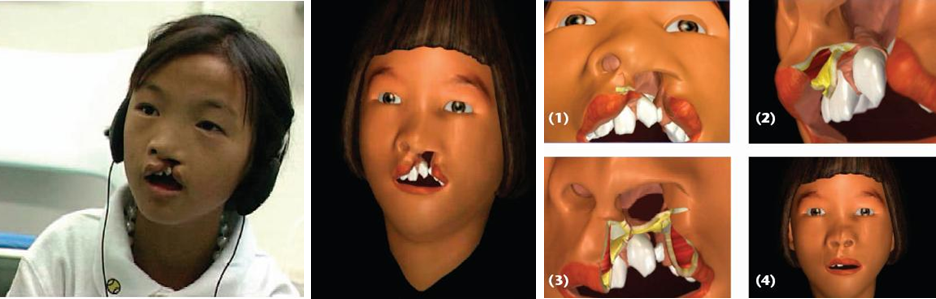
\includegraphics[width=\columnwidth]{images/cleft_lip_image}
\caption{Surgical simulation will ideally be used to provide a virtual environment of prototyping procedures as well as for research and development of novel procedures. The images show a subject specific simulated cleft lip and palate repair. Elastic simulation of soft tissues is the primary algorithmic challenge in providing such technologies.}
\end{figure}

\section*{Real-time computing}
Real-time simulation refers to the ability to evolve the approximation to an initial boundary value problem in less than a thirtieth of a second. In other words, less than the time it would take to observe the solution on the screen. Traditionally, computation times required for a time step in such problems have been on the order of a few minutes or even a few hours, far short of the thirtieth of a second constraint. However, such performance, should it be allowed, would provide a controllable virtual environment where a user would have the ability to change the forcing and boundary conditions of a simulation in response to real-time observation of the solution. The application of such functionality for solid and fluid mechanics problems is engendering many new applications. For example, imagine an interactive virtual environment where the user interacts with a finite element simulation of biomechanical soft tissues. The governing equations dictate how the tissues respond to external influence from the users. This predictive ability would allow the user to push, pull or even cut/excise portions of the tissue in real time with full confidence that the real life counterpart would behave similarly. This ability could potentially revolutionize the process of training surgical residents and medics by providing a cost effective and scientific alternative to expensive cadaver based training. Imagine the ability to know the outcome of a surgical procedure before it is performed. Reconstructive surgery for severe trauma is unpredictable by the nature of the injuries. The surgeon must design the treatment procedure on a case-by case-basis. With the aid of a predictive simulator the surgeon could perform hypothetical surgical repairs in advance to determine the most likely successful approach. This would significantly reduce complication rates and lead to drastically improved quality of life. See \cite{Sifakis09} for further discussion of the potential benefits of surgical simulation.
